\section{Hardware}

Hardware:
•	Arduino MKR WAN 1310
Already includes a LPWAN module called Murata CMWX1ZZABZ
Need to add an external antenna, the Arduino documentation suggests Dipole Pentaband Waterproof Antenna (https://store.arduino.cc/products/dipole-pentaband-waterproof-antenna).
•	DHT22 sensor: connected by a digital pin to the Arduino
•	LoRaWAN Gateway: we can search if we have a neraby gateway from The Things Network at https://www.thethingsnetwork.org/map. If that’s not the case, we will need to implement our own gatway. 
You can buy a LoRa Gateway online for indoor or outdoor usage, based on your needs, e.g. indoor (Mikrotik wAP LR8) outdoor (TEKTELIC KONA MACRO OUTDOOR GATEWAY).
Otherwise, you can build your own gateway, e.g. by using a Raspberry Pi 4, a  LoRa concentrator board, such as a RAK2245 Pi Hat, and an antenna.
•	Network Sever The Things Network
•	ThingSpeak
Describe…

Arduino and DHT22 are phisically connected.
Arduino communicates with the Gateway through LoRaWAN.
Gateway to TTN 
The Gateway can communicate with The Things Network with the gateway connector protocol, that uses as network protocol gRPC or MQTT.
TTN communicates the data to ThingSpeak through the built in integration, using the HTTP API exposed by ThingSpeak.

Software:
•	Codice Arduino 
•	Console TTN
•	Creazione channel 

\section{Software}
\label{sec:software}
In this section we present the software components used to allow the system to work. Since we don't own some hardware components, we were not able to test the whole system, but we tested individual components, as will be explained in the following sections.

\subsection{Code Arduino MKR WAN 1310}
The code that we will run on the Arduino MKR WAN 1310 is reported here.

\begin{lstlisting}[language=Arduino, numbers=none]
#include <MKRWAN.h>
#include <DHT.h>

#define DHTPIN 7
#define DHTTYPE DHT22
DHT dht(DHTPIN, DHTTYPE);

LoRaModem modem(Serial1);

// TTN credentials
String appEui = "0000000000000000";  
String appKey = "9D265EE3895BE505824143EBD5FDC46B";

void setup() {
  // initialization
  Serial.begin(115200);
  dht.begin();
  
  // LoRa module initialization
  if (!modem.begin(EU868)) {
    Serial.println("Errore avvio LoRa"); 
    while (1);
  }
  
  // join network server
  int connected = modem.joinOTAA(appEui, appKey);
  if (!connected) {
    Serial.println("- Something went wrong; are you indoor? Move near a window and retry...");
    while (1);
  }
}

void loop() {
  // read humidity and temperature
  float t = dht.readTemperature();
  float h = dht.readHumidity();
  
  // check readings 
  if (isnan(h) || isnan(t)) return;

  // encode readings
  byte payload[4];
  int16_t tt = t * 100;
  int16_t hh = h * 100;
  payload[0] = highByte(tt);
  payload[1] = lowByte(tt);
  payload[2] = highByte(hh);
  payload[3] = lowByte(hh);

  // send message
  modem.beginPacket();
  modem.write(payload, sizeof(payload));
  modem.endPacket();

  // send a reading every minute 
  delay(60000);
}
\end{lstlisting}

In the first line of the program, we include libraries needed to use LoRaWAN to communicate readings values and to use DHT22 sensor to measure temperature and humidity. Then, we define the digital PIN to which the DHT22 sensor is connected and the DHTTYPE, representing the sensor model. The code is formed by two functions: setup and loop. In setup, we initialize both the DHT22 and the LoRa communication, setting the Carrier Frequency to 868 MHz. Moreover, we join the network server thanks to the joinOTAA function. In the loop function, instead, we perform sensor readings for temperature and humidity, encode these values and send them over LoRaWAN netwok. Finally, we insert a delay of 1 minute to wait for the next reading and message.
	 
\subsection{The Things Network Console and ThingSpeak}
In this section, we provide a detailed explanation of all the work we have done to setup The Things Network (TTN) and ThingSpeak to make the system fully functional. We present all the steps in chronological order and add figures to document the result.
\subsubsection{Create an Application on TTN}
After creating an account on TTN, we created an Application and set the Application ID, a name and a description.

\begin{figure}[H]
    \centering
    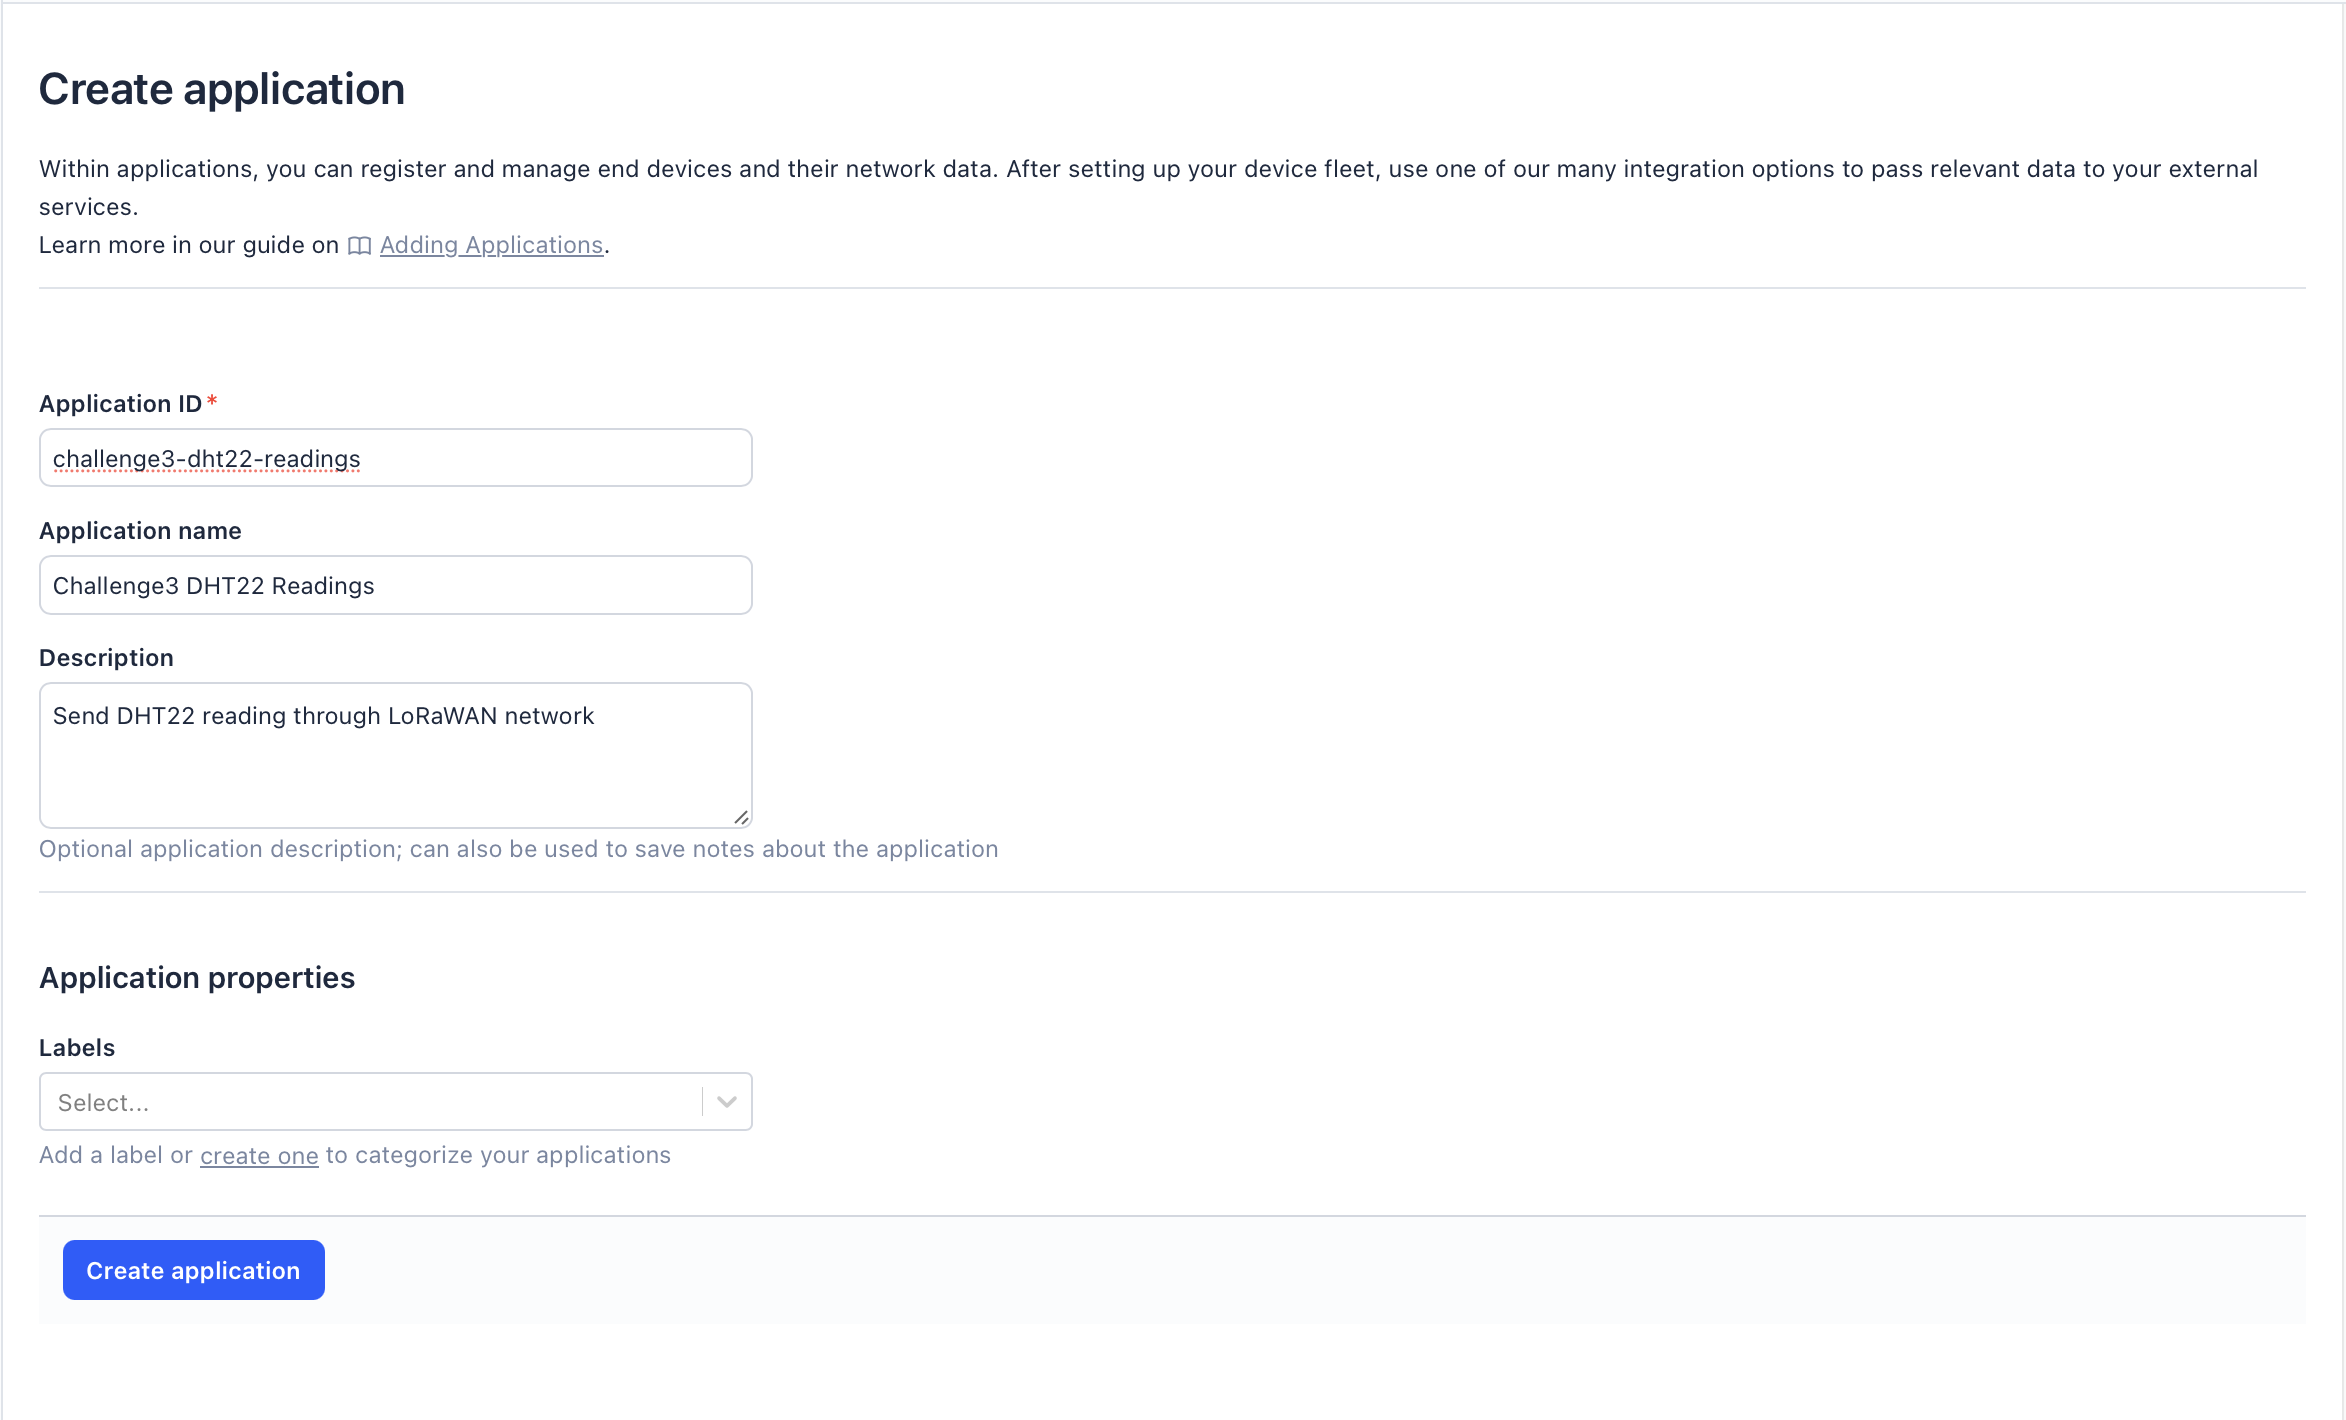
\includegraphics[width=0.8\linewidth, height=0.5\textheight, keepaspectratio]{create_application.png}
    \caption{Create an Application on TTN}
\end{figure}

\subsubsection{Generate an API key}
From the API keys section of TTN Console, we generated an API key for the newly created Application.

\begin{figure}[H]
    \centering
    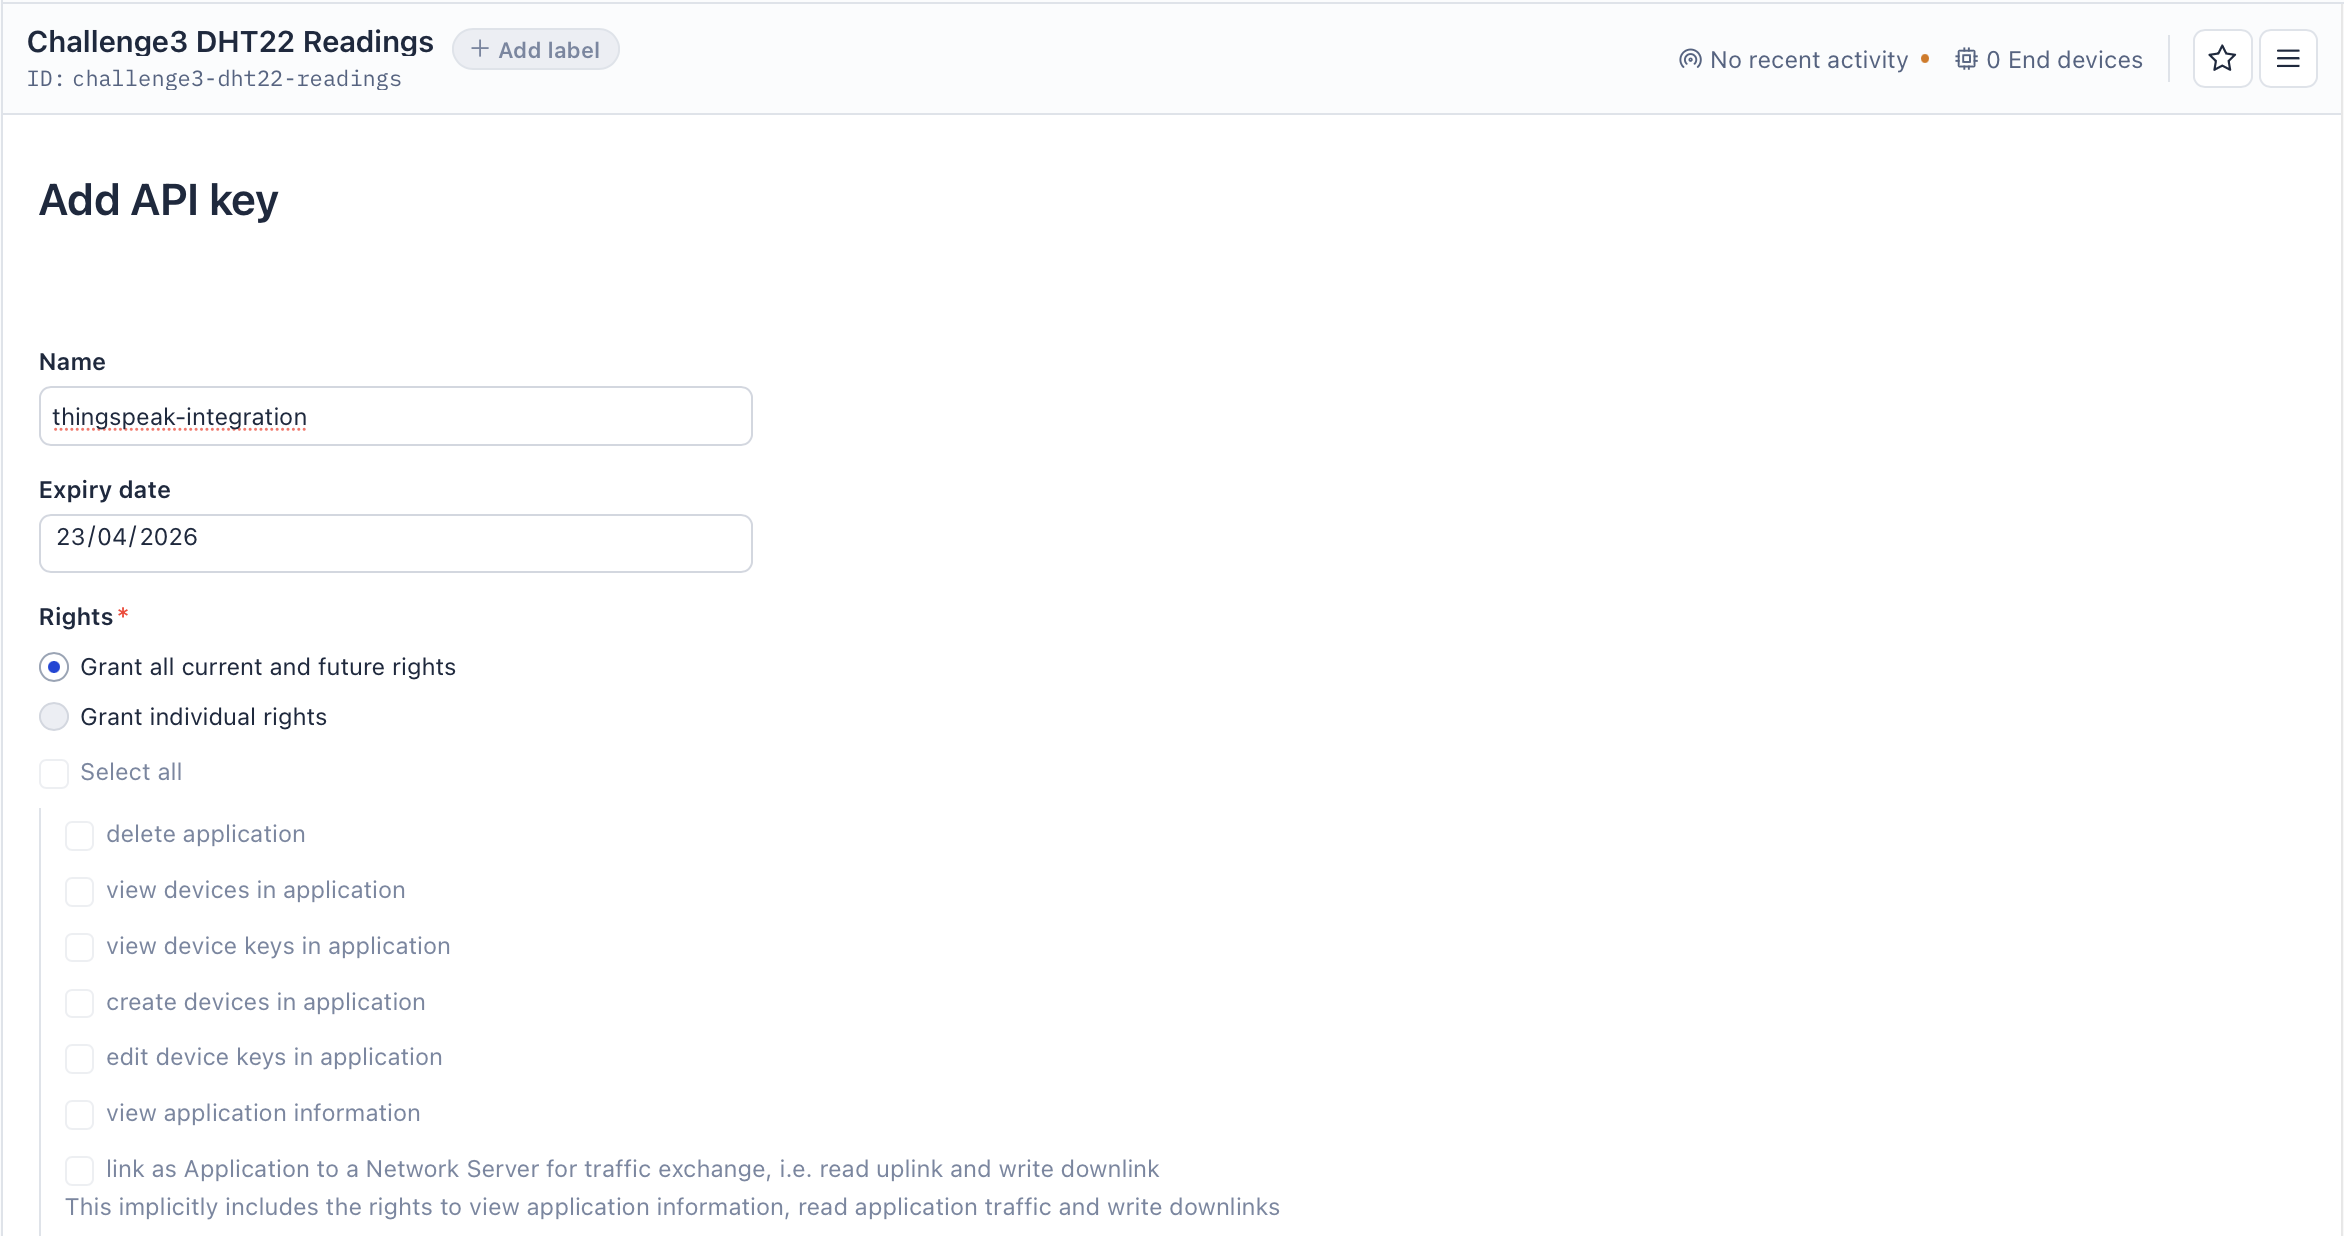
\includegraphics[width=0.8\linewidth, height=0.5\textheight, keepaspectratio]{generate_api_key.png}
    \caption{Generate an API key}
\end{figure}

\subsubsection{Register Arduino MKR WAN 1310 End Device}
In the End devices section of TTN Console, we added the Arduino MKR WAN 1310 End Device by setting the brand, the model and other details about the board, as well as the recommended frequency plan. 

\begin{figure}[H]
    \centering
    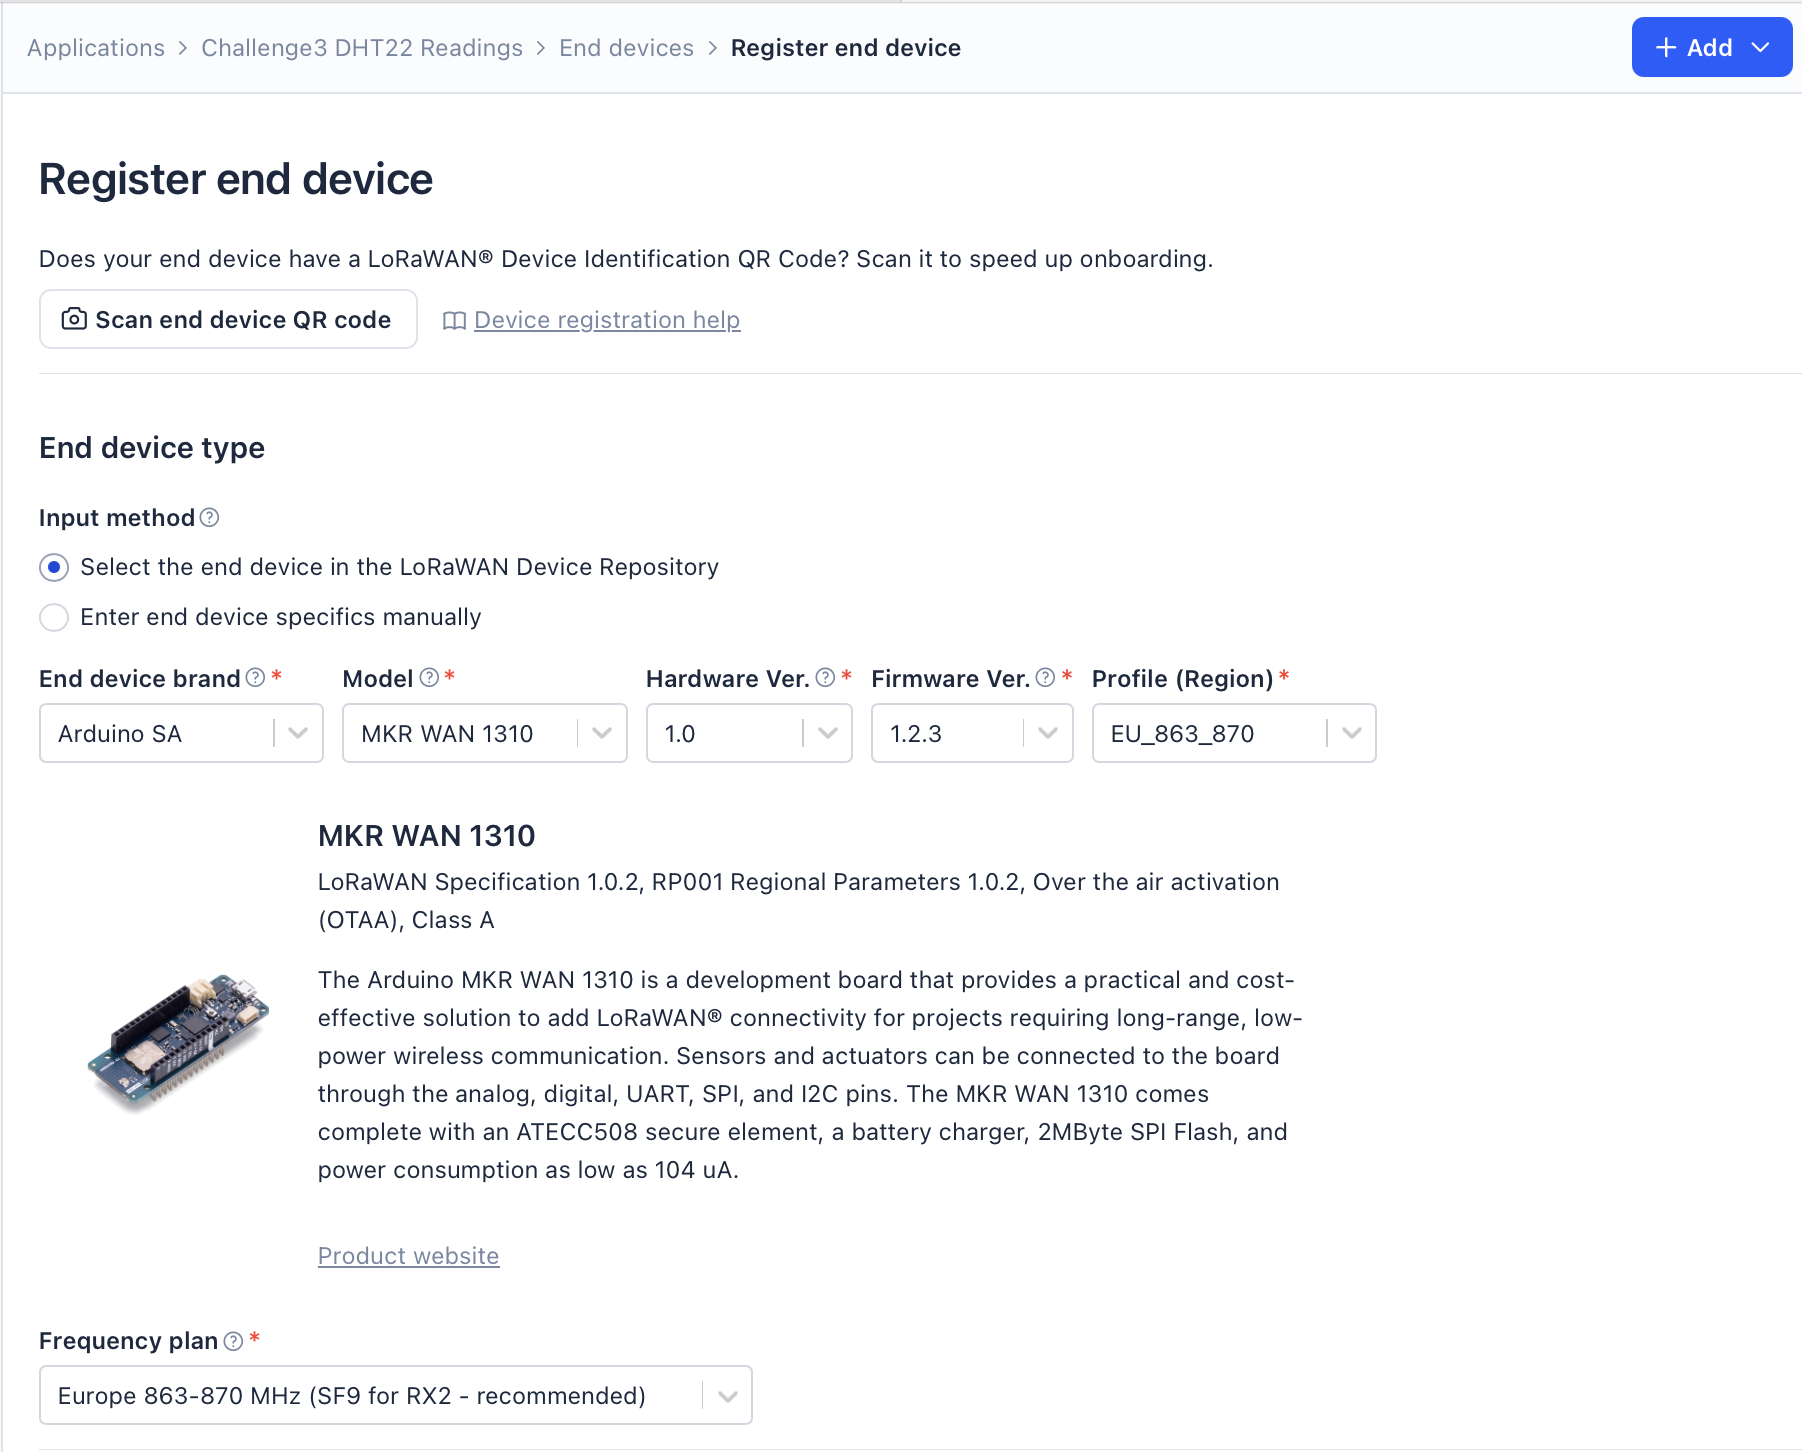
\includegraphics[width=0.8\linewidth, height=0.5\textheight, keepaspectratio]{register_end_device_1.png}
    \caption{Register an end device part 1}
\end{figure}

We also generated the AppKey, AppEUI and DevEUI, some of these values are chosen arbitrarily, because we don't have the real Arduino board.

\begin{figure}[H]
    \centering
    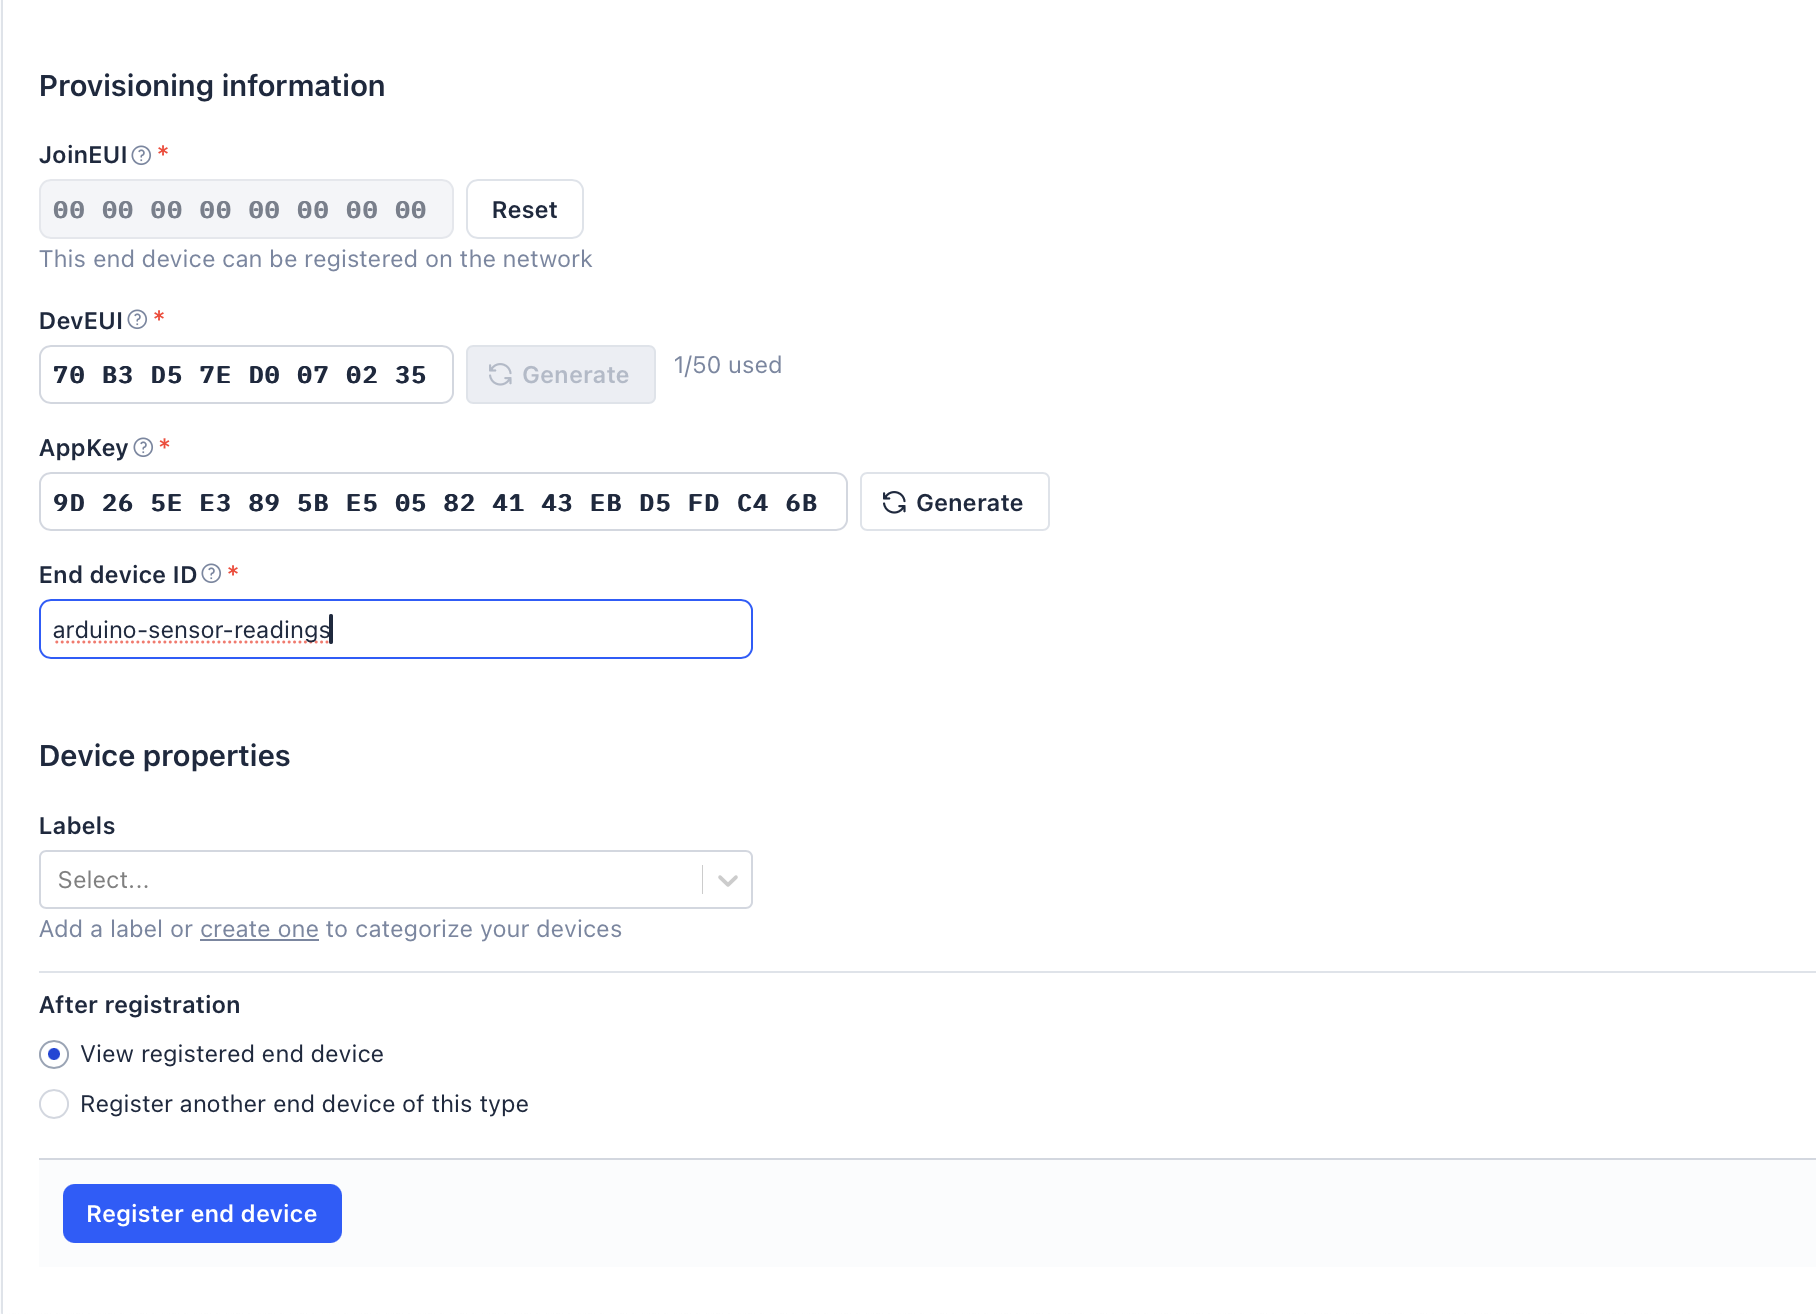
\includegraphics[width=0.8\linewidth, height=0.5\textheight, keepaspectratio]{register_end_device_2.png}
    \caption{Register an end device part 2}
\end{figure}

\subsubsection{Configure Uplink Payload Formatter}
We configured the uplink payload formatter to decode the data coming from the Arduino board. We chose a custom JavaScript formatter and wrote the JS code that decodes the data in the same way we have encoded it in the Arduino code. We return a JS object that has the correct format for the integration with ThingSpeak, as shown in the following figure.

\begin{figure}[H]
    \centering
    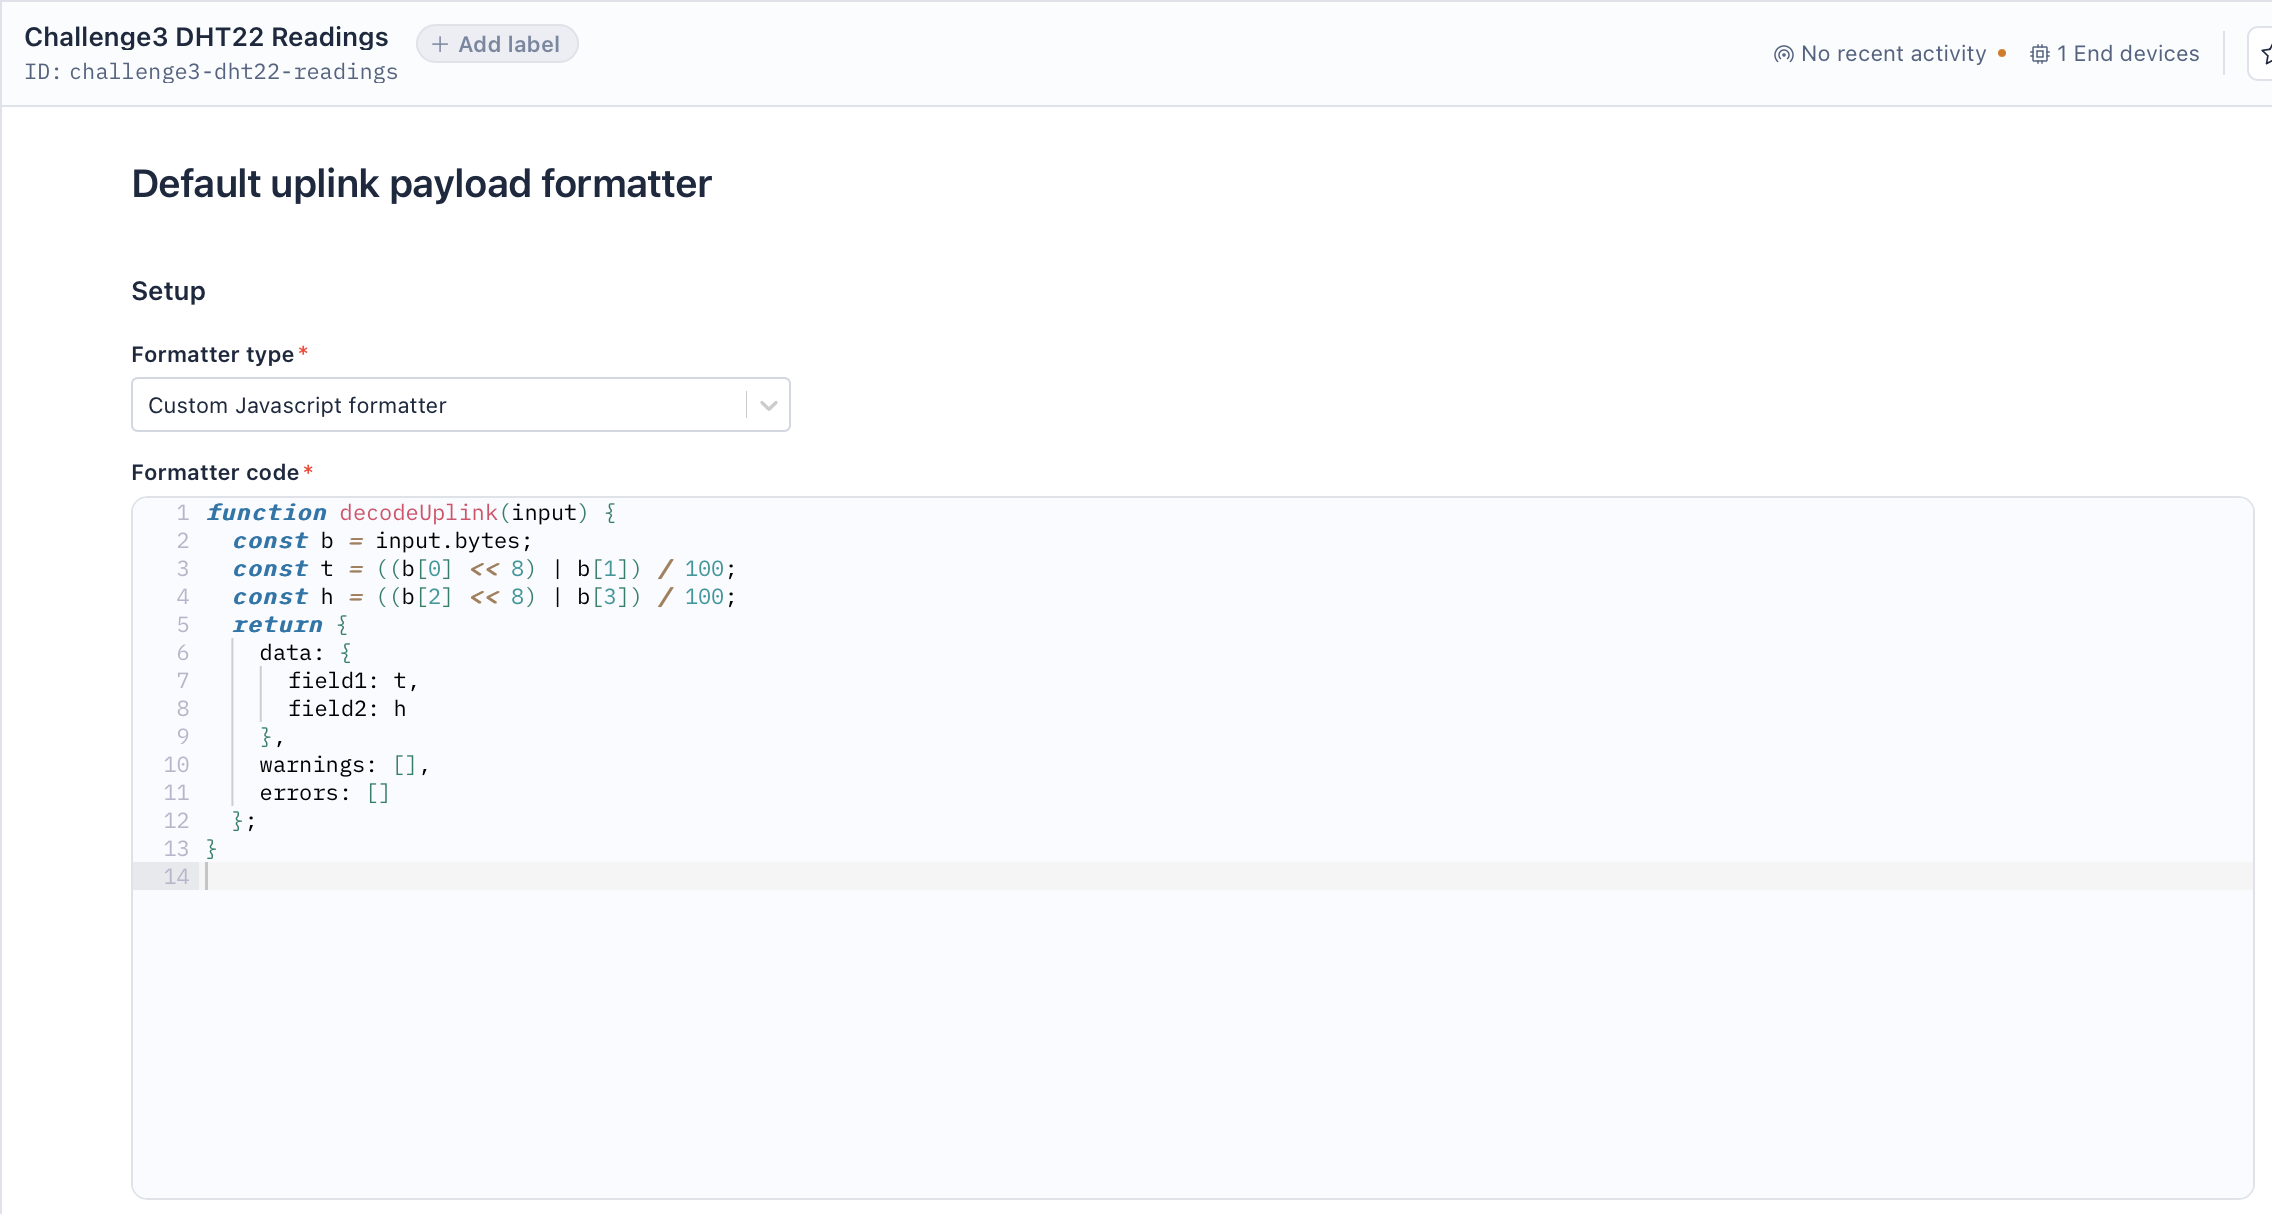
\includegraphics[width=0.8\linewidth, height=0.5\textheight, keepaspectratio]{uplink_formatter.png}
    \caption{Configure Uplink Payload Formatter}
\end{figure}

\subsubsection{Create ThingSpeak Channel}
We created the ThingSpeak Channel that receives the temperature and humidity values from TTN. We assigned a name and a description to the channel and we create the two desired fields. Finally we made it publicly available at \url{https://thingspeak.mathworks.com/channels/2931560}.

\begin{figure}[H]
    \centering
    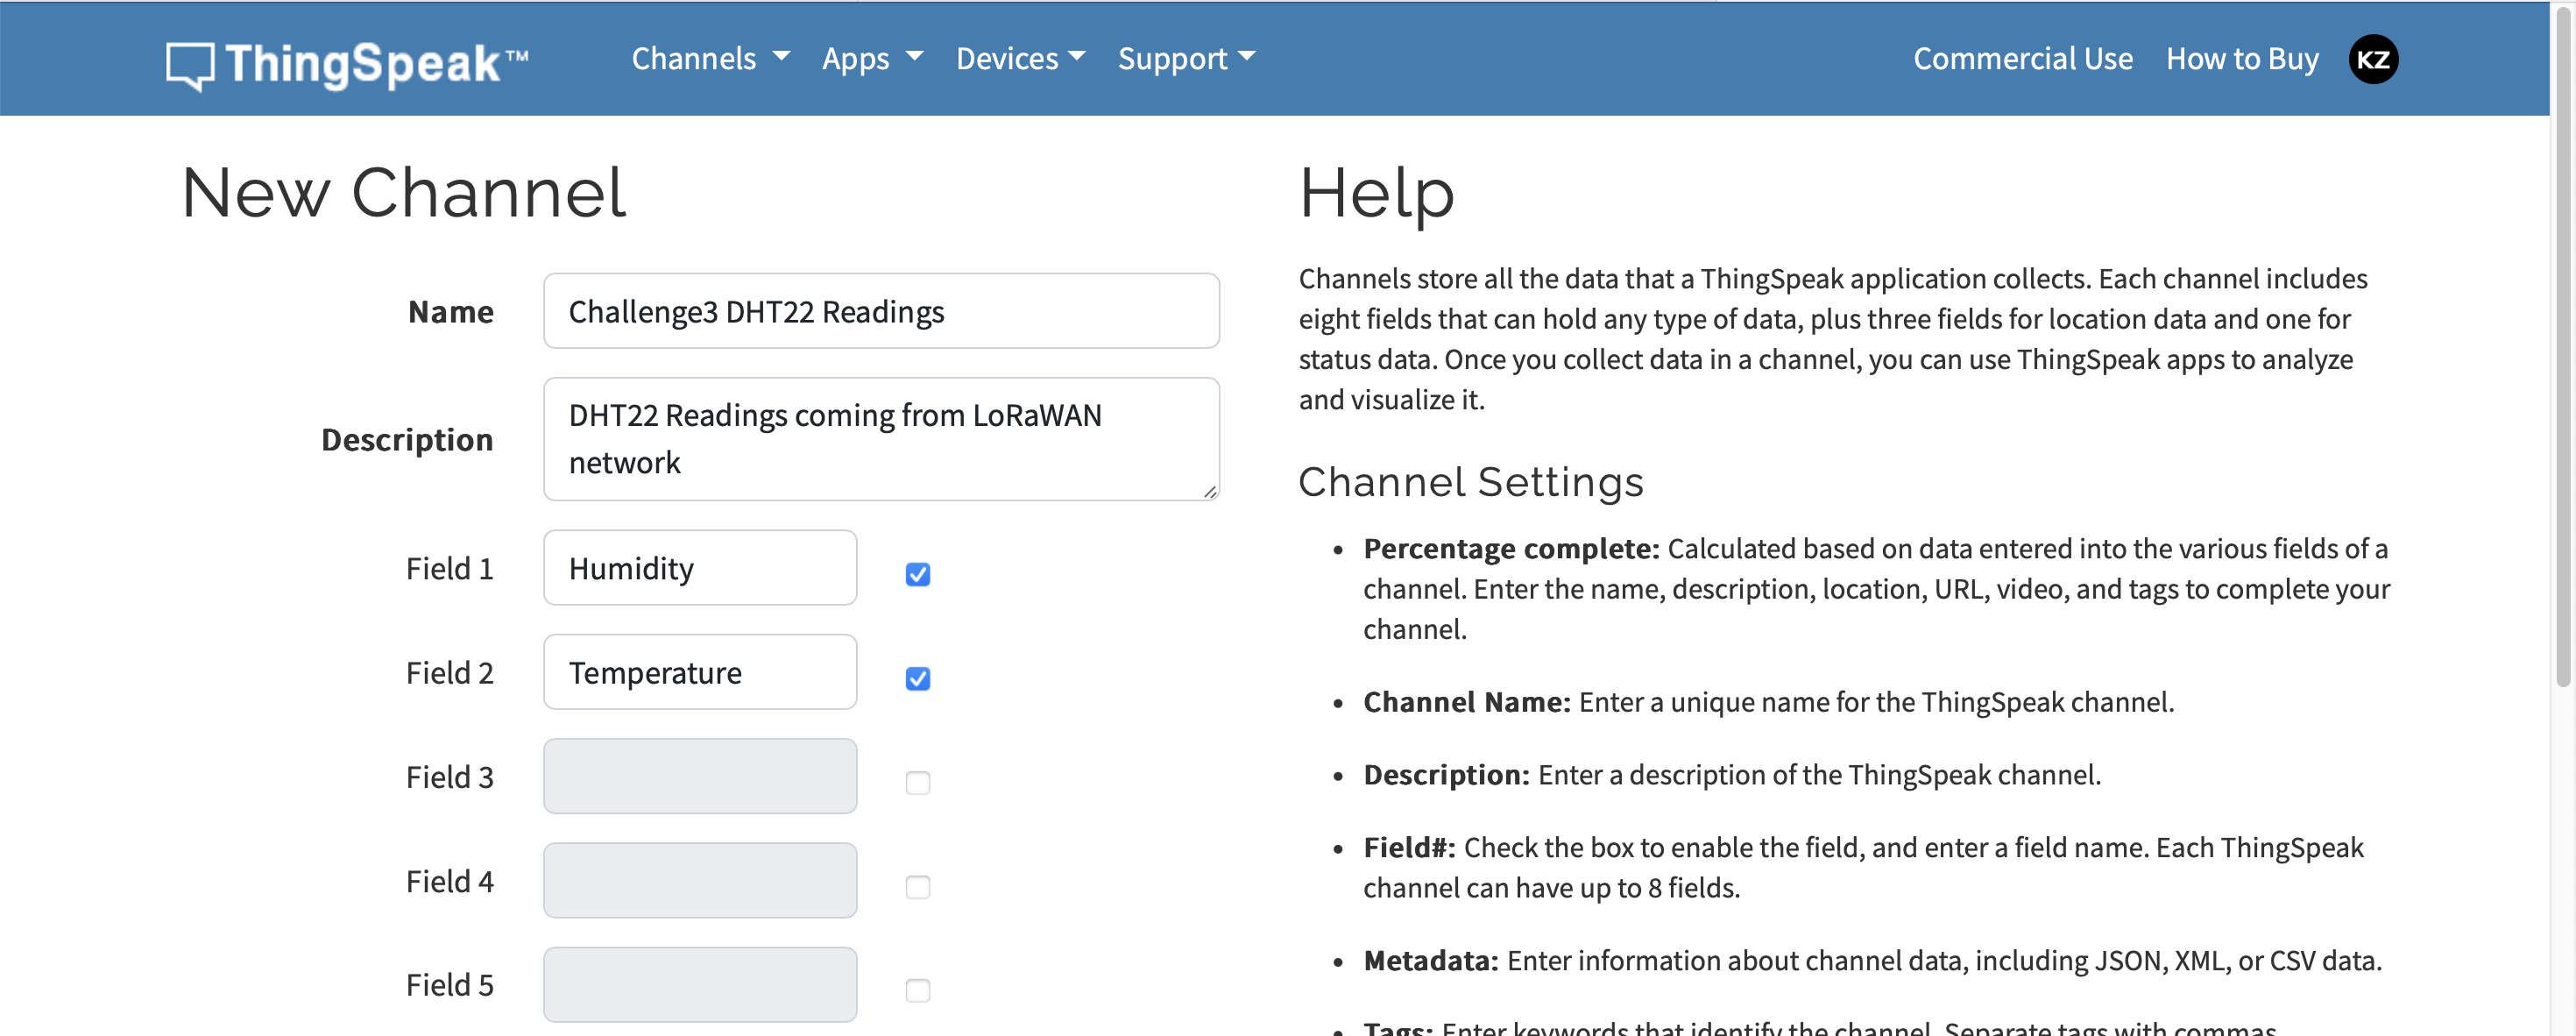
\includegraphics[width=0.8\linewidth, height=0.5\textheight, keepaspectratio]{new_channel.png}
    \caption{Create ThingSpeak Channel}
\end{figure}

\subsubsection{Integrating The Things Network and ThingSpeak}
In order to integrate TTN and ThingSpeak, we setup a webhook for ThingSpeak and insert the Channel ID and write API Key, which we take from ThingSpeak.

\begin{figure}[H]
    \centering
    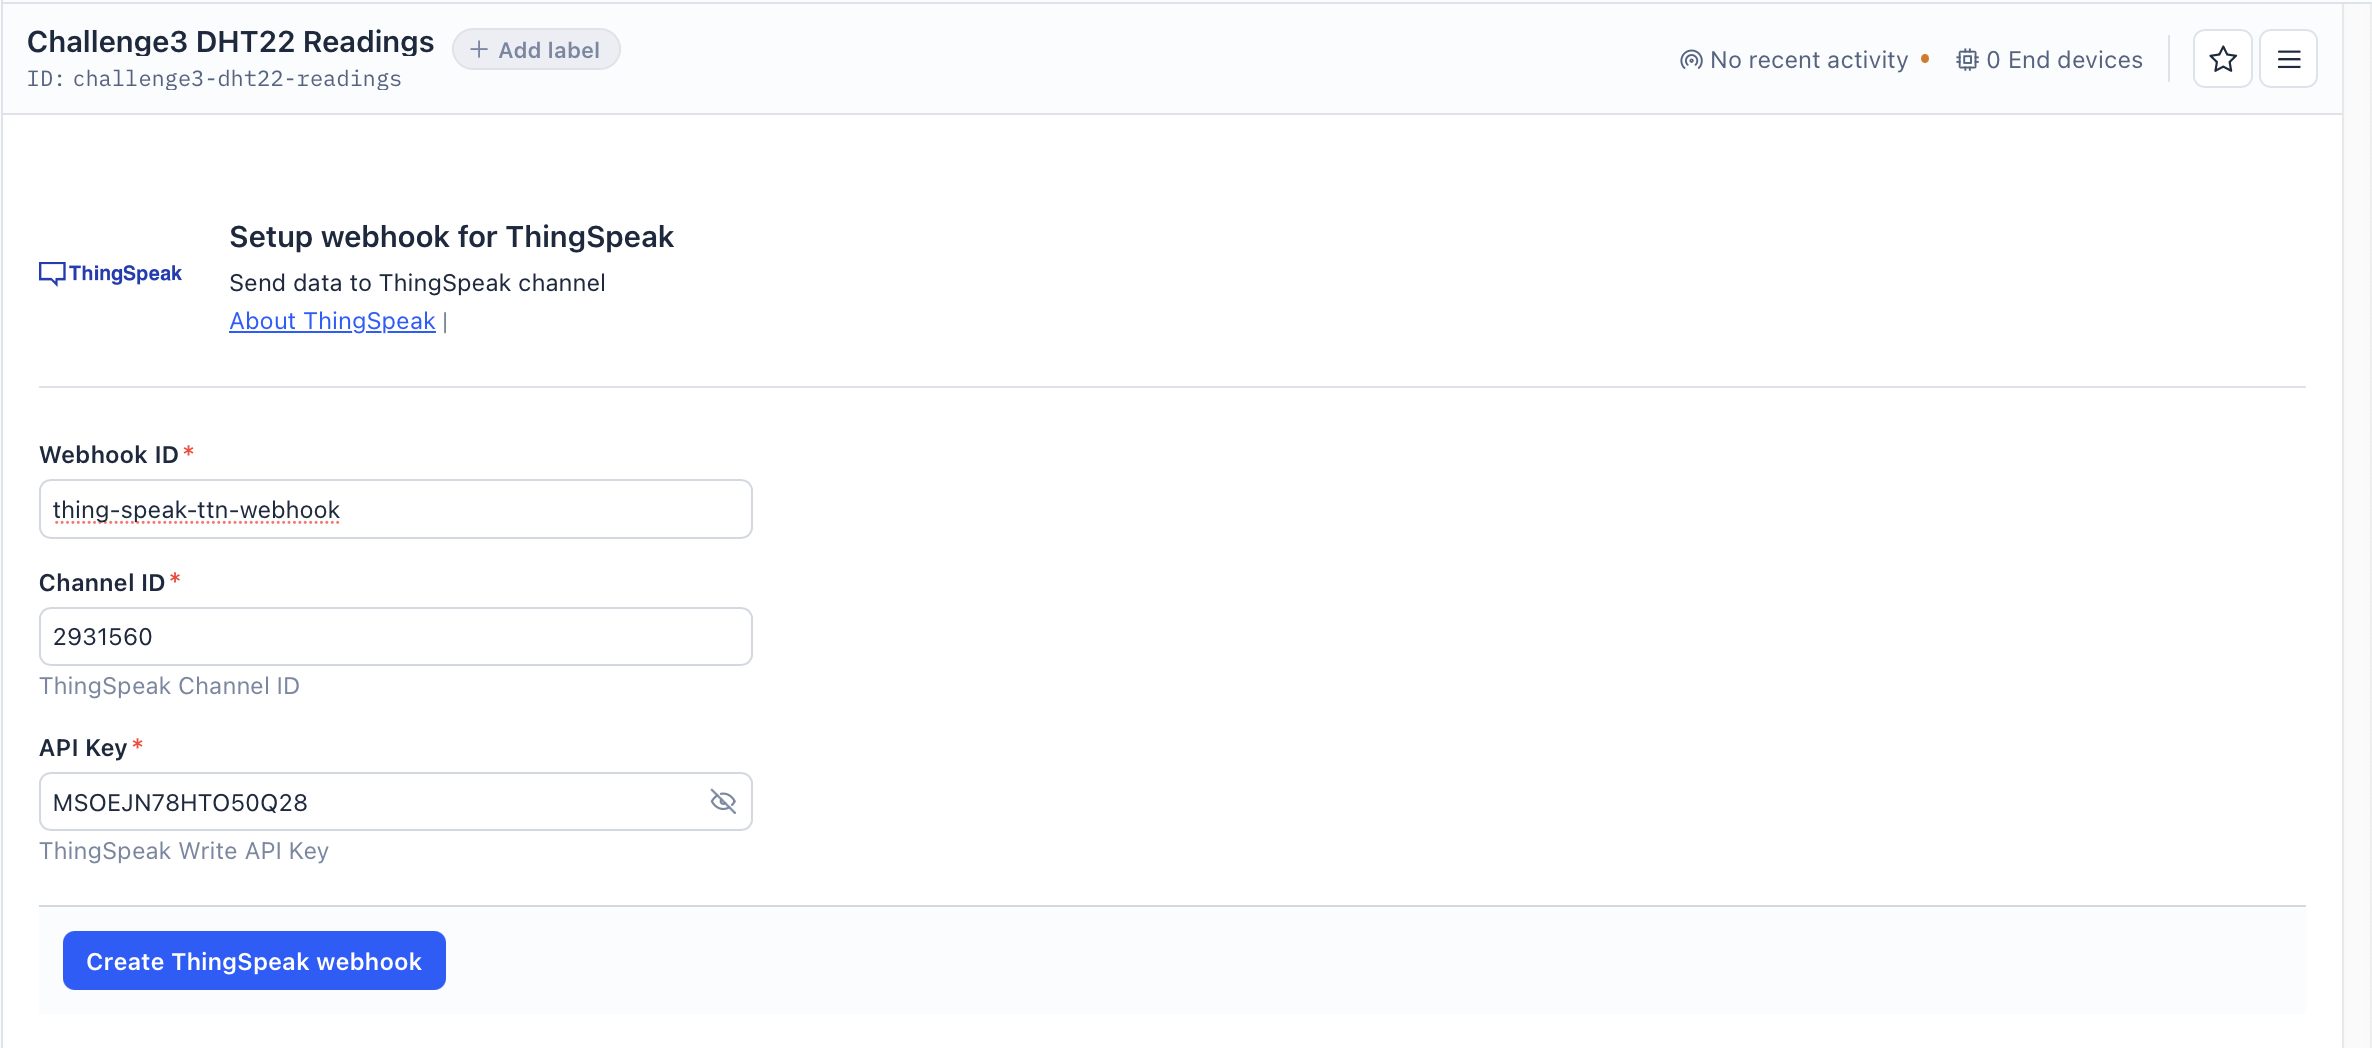
\includegraphics[width=0.8\linewidth, height=0.5\textheight, keepaspectratio]{webhook.png}
    \caption{Integrating TTN and ThingSpeak}
\end{figure}

\subsection{Test TTN and ThingSpeakIntegration}
Finally, we used test payload function of TTN to send some test payloads to ThingSpeak and test the integration between the two.

\begin{figure}[H]
    \centering
    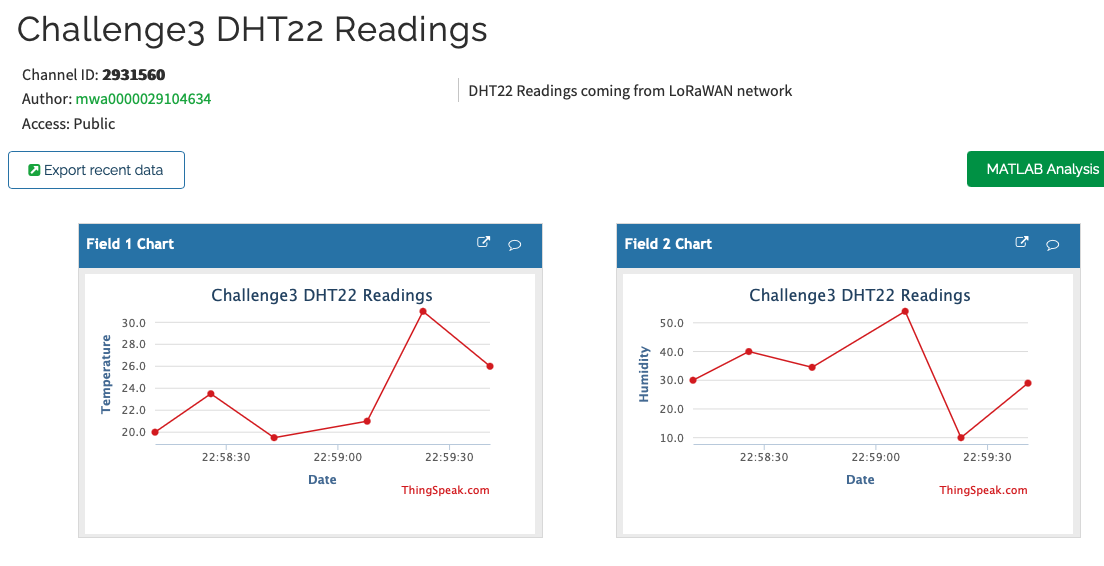
\includegraphics[width=0.8\linewidth, height=0.5\textheight, keepaspectratio]{thingspeak_charts.png}
    \caption{ThingSpeak fields charts}
\end{figure}




